% Options for packages loaded elsewhere
\PassOptionsToPackage{unicode}{hyperref}
\PassOptionsToPackage{hyphens}{url}
%
\documentclass[
]{article}
\usepackage{amsmath,amssymb}
\usepackage{iftex}
\ifPDFTeX
  \usepackage[T1]{fontenc}
  \usepackage[utf8]{inputenc}
  \usepackage{textcomp} % provide euro and other symbols
\else % if luatex or xetex
  \usepackage{unicode-math} % this also loads fontspec
  \defaultfontfeatures{Scale=MatchLowercase}
  \defaultfontfeatures[\rmfamily]{Ligatures=TeX,Scale=1}
\fi
\usepackage{lmodern}
\ifPDFTeX\else
  % xetex/luatex font selection
\fi
% Use upquote if available, for straight quotes in verbatim environments
\IfFileExists{upquote.sty}{\usepackage{upquote}}{}
\IfFileExists{microtype.sty}{% use microtype if available
  \usepackage[]{microtype}
  \UseMicrotypeSet[protrusion]{basicmath} % disable protrusion for tt fonts
}{}
\makeatletter
\@ifundefined{KOMAClassName}{% if non-KOMA class
  \IfFileExists{parskip.sty}{%
    \usepackage{parskip}
  }{% else
    \setlength{\parindent}{0pt}
    \setlength{\parskip}{6pt plus 2pt minus 1pt}}
}{% if KOMA class
  \KOMAoptions{parskip=half}}
\makeatother
\usepackage{xcolor}
\usepackage{color}
\usepackage{fancyvrb}
\newcommand{\VerbBar}{|}
\newcommand{\VERB}{\Verb[commandchars=\\\{\}]}
\DefineVerbatimEnvironment{Highlighting}{Verbatim}{commandchars=\\\{\}}
% Add ',fontsize=\small' for more characters per line
\newenvironment{Shaded}{}{}
\newcommand{\AlertTok}[1]{\textcolor[rgb]{1.00,0.00,0.00}{\textbf{#1}}}
\newcommand{\AnnotationTok}[1]{\textcolor[rgb]{0.38,0.63,0.69}{\textbf{\textit{#1}}}}
\newcommand{\AttributeTok}[1]{\textcolor[rgb]{0.49,0.56,0.16}{#1}}
\newcommand{\BaseNTok}[1]{\textcolor[rgb]{0.25,0.63,0.44}{#1}}
\newcommand{\BuiltInTok}[1]{\textcolor[rgb]{0.00,0.50,0.00}{#1}}
\newcommand{\CharTok}[1]{\textcolor[rgb]{0.25,0.44,0.63}{#1}}
\newcommand{\CommentTok}[1]{\textcolor[rgb]{0.38,0.63,0.69}{\textit{#1}}}
\newcommand{\CommentVarTok}[1]{\textcolor[rgb]{0.38,0.63,0.69}{\textbf{\textit{#1}}}}
\newcommand{\ConstantTok}[1]{\textcolor[rgb]{0.53,0.00,0.00}{#1}}
\newcommand{\ControlFlowTok}[1]{\textcolor[rgb]{0.00,0.44,0.13}{\textbf{#1}}}
\newcommand{\DataTypeTok}[1]{\textcolor[rgb]{0.56,0.13,0.00}{#1}}
\newcommand{\DecValTok}[1]{\textcolor[rgb]{0.25,0.63,0.44}{#1}}
\newcommand{\DocumentationTok}[1]{\textcolor[rgb]{0.73,0.13,0.13}{\textit{#1}}}
\newcommand{\ErrorTok}[1]{\textcolor[rgb]{1.00,0.00,0.00}{\textbf{#1}}}
\newcommand{\ExtensionTok}[1]{#1}
\newcommand{\FloatTok}[1]{\textcolor[rgb]{0.25,0.63,0.44}{#1}}
\newcommand{\FunctionTok}[1]{\textcolor[rgb]{0.02,0.16,0.49}{#1}}
\newcommand{\ImportTok}[1]{\textcolor[rgb]{0.00,0.50,0.00}{\textbf{#1}}}
\newcommand{\InformationTok}[1]{\textcolor[rgb]{0.38,0.63,0.69}{\textbf{\textit{#1}}}}
\newcommand{\KeywordTok}[1]{\textcolor[rgb]{0.00,0.44,0.13}{\textbf{#1}}}
\newcommand{\NormalTok}[1]{#1}
\newcommand{\OperatorTok}[1]{\textcolor[rgb]{0.40,0.40,0.40}{#1}}
\newcommand{\OtherTok}[1]{\textcolor[rgb]{0.00,0.44,0.13}{#1}}
\newcommand{\PreprocessorTok}[1]{\textcolor[rgb]{0.74,0.48,0.00}{#1}}
\newcommand{\RegionMarkerTok}[1]{#1}
\newcommand{\SpecialCharTok}[1]{\textcolor[rgb]{0.25,0.44,0.63}{#1}}
\newcommand{\SpecialStringTok}[1]{\textcolor[rgb]{0.73,0.40,0.53}{#1}}
\newcommand{\StringTok}[1]{\textcolor[rgb]{0.25,0.44,0.63}{#1}}
\newcommand{\VariableTok}[1]{\textcolor[rgb]{0.10,0.09,0.49}{#1}}
\newcommand{\VerbatimStringTok}[1]{\textcolor[rgb]{0.25,0.44,0.63}{#1}}
\newcommand{\WarningTok}[1]{\textcolor[rgb]{0.38,0.63,0.69}{\textbf{\textit{#1}}}}
\usepackage{graphicx}
\makeatletter
\def\maxwidth{\ifdim\Gin@nat@width>\linewidth\linewidth\else\Gin@nat@width\fi}
\def\maxheight{\ifdim\Gin@nat@height>\textheight\textheight\else\Gin@nat@height\fi}
\makeatother
% Scale images if necessary, so that they will not overflow the page
% margins by default, and it is still possible to overwrite the defaults
% using explicit options in \includegraphics[width, height, ...]{}
\setkeys{Gin}{width=\maxwidth,height=\maxheight,keepaspectratio}
% Set default figure placement to htbp
\makeatletter
\def\fps@figure{htbp}
\makeatother
\usepackage{svg}
\setlength{\emergencystretch}{3em} % prevent overfull lines
\providecommand{\tightlist}{%
  \setlength{\itemsep}{0pt}\setlength{\parskip}{0pt}}
\setcounter{secnumdepth}{-\maxdimen} % remove section numbering
\ifLuaTeX
  \usepackage{selnolig}  % disable illegal ligatures
\fi
\IfFileExists{bookmark.sty}{\usepackage{bookmark}}{\usepackage{hyperref}}
\IfFileExists{xurl.sty}{\usepackage{xurl}}{} % add URL line breaks if available
\urlstyle{same}
\hypersetup{
  hidelinks,
  pdfcreator={LaTeX via pandoc}}

\author{}
\date{}

\begin{document}

\hypertarget{full-adder-simulations-report}{%
\section{Full Adder Simulations
Report}\label{full-adder-simulations-report}}

\hypertarget{introduction}{%
\section{Introduction}\label{introduction}}

In this lab, I built full adder simulations in \texttt{Vivado} software,
involving behavioral simulation, post-synthesis functional simulation,
post-synthesis timing simulation, post-implement functional simulation,
and post-implement timing simulation. After these elaborate simulations,
I had a better understanding of the basics of digital system design. In
short, digital system design is quite different from developing
software, which not only requires us to write feasible and logical code
but also requires us to have physical hardware in mind. The most
significant difference is that concurrent statements are the main
components in a \texttt{VHDL} file, which means the statements do not
execute line by line. Due to the physical constraints on board, I also
understand that not all designs are synthesizable or implementable, and
even if one design is capable of being synthesized, it may appear
different behaviors in different simulation stages.

\hypertarget{prerequisite}{%
\section{Prerequisite}\label{prerequisite}}

This lab focuses on full adder, so let's first analyze a full adder
using Boolean algebra.

Basically, a full adder can be described in the following Boolean
expression:

\begin{align*}
s1&=A\oplus B\\
s2&=Cin\times s1\\
s3&=A\times B\\
sum&=s1\oplus Cin\\
cout&=s2 + s3\\
\end{align*}

This expression can be transferred to an equivalent logic diagram
(Figure TODO):\\
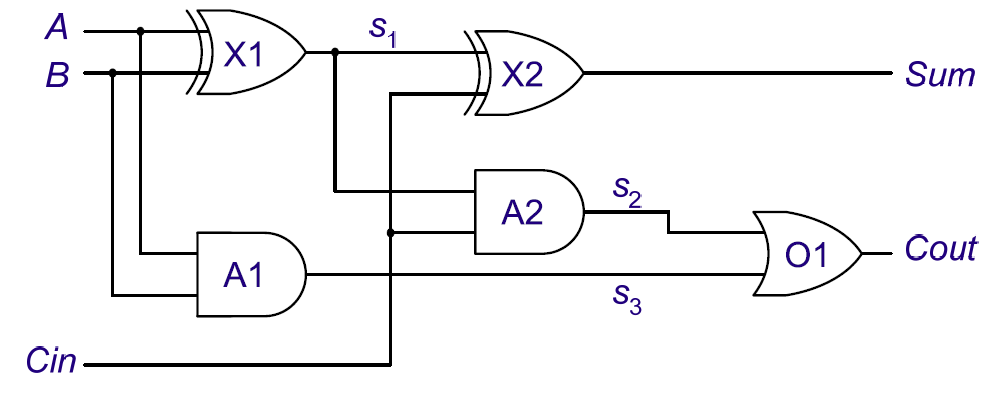
\includegraphics{D:/MyProjects/FPGA/Lab2/full_addr_report/assets/image-20240306101306521.png}

where \(A\) and \(B\) are two one-bit inputs, \(Cin\) is the carry bit
of the previous bit full adder (i.e. \(Cout\) of the previous full
adder). \(s1\), \(s2\) and \(s3\) are intermediate signals.

When applying the stimulus signals like Figure TODO, using the Boolean
algebra, we can then manually derive the timing diagram (Figure TODO) of
the above logic diagram. The timing diagram uses \emph{Wavedrom editor}
to generate.

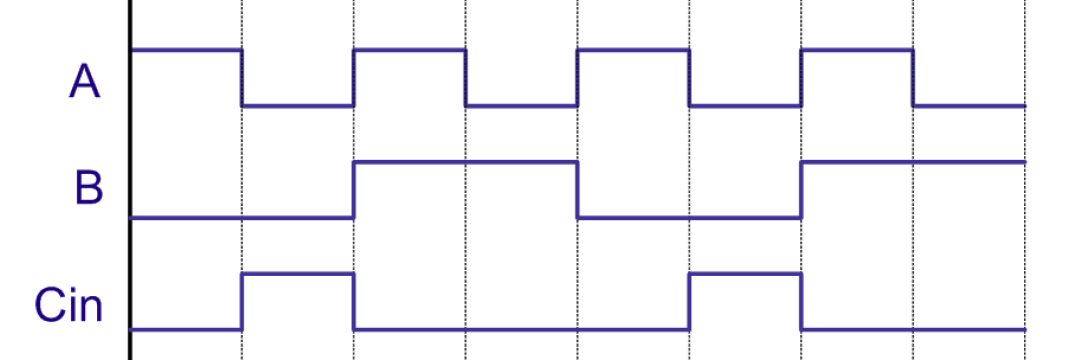
\includegraphics{D:/MyProjects/FPGA/Lab2/full_addr_report/assets/image-20240306190552572.png}

\includesvg{D:/MyProjects/FPGA/Lab2/full_addr_report/assets/wavedrom.svg}

\textbf{Note that}, we added a 10ns of gate delay to all the gates
above. Every grid represents 10ns. The dotted line in the signal means
at this time, the signal is not yet initialized. In this timing diagram,
the intermediate signals as well as the output signals are represented
in a slow-variation fashion (i.e. there is a ramp when the signal jumps
from 0 to 1 or vice versa).

\hypertarget{source-code-analysis}{%
\section{Source Code Analysis}\label{source-code-analysis}}

\hypertarget{design-source}{%
\subsection{Design Source}\label{design-source}}

Describing the logic diagram in \texttt{VHDL} language is easy, the core
part of the full adder's code is almost a direct translation of the
Boolean expression.

\begin{Shaded}
\begin{Highlighting}[]
\ControlFlowTok{architecture} \DecValTok{dataflow} \KeywordTok{of} \FunctionTok{full\_addr} \KeywordTok{is}
    \OtherTok{signal}\NormalTok{ s1}\OtherTok{,}\NormalTok{ s2}\OtherTok{,}\NormalTok{ s3 }\OtherTok{:} \DataTypeTok{std\_logic}\NormalTok{;}
    \OtherTok{constant}\NormalTok{ gate\_delay }\OtherTok{:} \DataTypeTok{time} \OtherTok{:=} \DecValTok{10} \DataTypeTok{ns}\NormalTok{;}
\ControlFlowTok{begin}
    \DecValTok{L1}\OtherTok{:} \FunctionTok{s1} \OtherTok{\textless{}=}\NormalTok{ (A }\KeywordTok{xor}\NormalTok{ B) }\KeywordTok{after}\NormalTok{ gate\_delay;}
    \DecValTok{L2}\OtherTok{:} \FunctionTok{s2} \OtherTok{\textless{}=}\NormalTok{ (Cin }\KeywordTok{and}\NormalTok{ s1) }\KeywordTok{after}\NormalTok{ gate\_delay;}
    \DecValTok{L3}\OtherTok{:} \FunctionTok{s3} \OtherTok{\textless{}=}\NormalTok{ (A }\KeywordTok{and}\NormalTok{ B) }\KeywordTok{after}\NormalTok{ gate\_delay;}
    \DecValTok{L4}\OtherTok{:} \FunctionTok{sum} \OtherTok{\textless{}=}\NormalTok{ (s1 }\KeywordTok{xor}\NormalTok{ Cin) }\KeywordTok{after}\NormalTok{ gate\_delay;}
    \DecValTok{L5}\OtherTok{:} \FunctionTok{cout} \OtherTok{\textless{}=}\NormalTok{ (s2 }\KeywordTok{or}\NormalTok{ s3) }\KeywordTok{after}\NormalTok{ gate\_delay;}
\ControlFlowTok{end architecture dataflow;}
\end{Highlighting}
\end{Shaded}

We set the \texttt{gate\_delay} explicitly here as 10ns.

\hypertarget{testbench}{%
\subsection{Testbench}\label{testbench}}

Testbench is a kind of special \texttt{.vhd} file, which is used to
verify the design source. Typically, a testbench doesn't have any
input/output port, and it treats the design source as a kind of
\emph{blackbox} component. It applies self-defined stimulus signals and
measures the output of the \emph{blackbox}.

To treat the design source as a component, we need to first declare the
input/output port of the full\_adder like the code below:

\begin{Shaded}
\begin{Highlighting}[]
    \ControlFlowTok{component} \DecValTok{full\_addr} \KeywordTok{is} 
        \ControlFlowTok{port}\NormalTok{(A}\OtherTok{,}\NormalTok{ B}\OtherTok{,}\NormalTok{ Cin }\OtherTok{:} \KeywordTok{in} \DataTypeTok{std\_logic}\NormalTok{;}
\NormalTok{             Sum}\OtherTok{,}\NormalTok{ Cout }\OtherTok{:} \KeywordTok{out} \DataTypeTok{std\_logic}\NormalTok{);}
    \ControlFlowTok{end component full\_addr;}
\end{Highlighting}
\end{Shaded}

Then in the body of the architecture, we instantiated the full adder
component.

\begin{Shaded}
\begin{Highlighting}[]
\NormalTok{    UUT }\OtherTok{:}\NormalTok{ full\_addr }\KeywordTok{port} \KeywordTok{map}\NormalTok{ (A}\OtherTok{=\textgreater{}}\NormalTok{A\_tb}\OtherTok{,}\NormalTok{ B}\OtherTok{=\textgreater{}}\NormalTok{B\_tb}\OtherTok{,}\NormalTok{ Cin}\OtherTok{=\textgreater{}}\NormalTok{Cin\_tb}\OtherTok{,}\NormalTok{ Sum}\OtherTok{=\textgreater{}}\NormalTok{Sum\_tb}\OtherTok{,}\NormalTok{ Cout}\OtherTok{=\textgreater{}}\NormalTok{Cout\_tb);}
\end{Highlighting}
\end{Shaded}

After the \emph{blackbox} is ready, we design the stimulus signals as
Figure TODO, using a naive implementation shown in the below code:

\begin{Shaded}
\begin{Highlighting}[]
    \CommentTok{{-}{-} Define stimulus signal}
\NormalTok{    A\_tb }\OtherTok{\textless{}=} \BaseNTok{\textquotesingle{}1\textquotesingle{}}\OtherTok{,} \BaseNTok{\textquotesingle{}0\textquotesingle{}} \KeywordTok{after}\NormalTok{ 10ns}\OtherTok{,} \BaseNTok{\textquotesingle{}1\textquotesingle{}} \KeywordTok{after}\NormalTok{ 20ns}\OtherTok{,}\BaseNTok{\textquotesingle{}0\textquotesingle{}} \KeywordTok{after}\NormalTok{ 30ns}\OtherTok{,} \BaseNTok{\textquotesingle{}1\textquotesingle{}} \KeywordTok{after}\NormalTok{ 40ns}\OtherTok{,}\BaseNTok{\textquotesingle{}0\textquotesingle{}} \KeywordTok{after}\NormalTok{ 50ns}\OtherTok{,} \BaseNTok{\textquotesingle{}1\textquotesingle{}} \KeywordTok{after}\NormalTok{ 60ns}\OtherTok{,}\BaseNTok{\textquotesingle{}0\textquotesingle{}} \KeywordTok{after}\NormalTok{ 70ns;}
\NormalTok{    B\_tb }\OtherTok{\textless{}=} \BaseNTok{\textquotesingle{}0\textquotesingle{}}\OtherTok{,} \BaseNTok{\textquotesingle{}1\textquotesingle{}} \KeywordTok{after}\NormalTok{ 20ns}\OtherTok{,} \BaseNTok{\textquotesingle{}0\textquotesingle{}} \KeywordTok{after}\NormalTok{ 40ns}\OtherTok{,} \BaseNTok{\textquotesingle{}1\textquotesingle{}} \KeywordTok{after}\NormalTok{ 60ns;}
\NormalTok{    Cin\_tb }\OtherTok{\textless{}=} \BaseNTok{\textquotesingle{}0\textquotesingle{}}\OtherTok{,} \BaseNTok{\textquotesingle{}1\textquotesingle{}} \KeywordTok{after}\NormalTok{ 10ns}\OtherTok{,} \BaseNTok{\textquotesingle{}0\textquotesingle{}} \KeywordTok{after}\NormalTok{ 20ns}\OtherTok{,} \BaseNTok{\textquotesingle{}1\textquotesingle{}} \KeywordTok{after}\NormalTok{ 50ns}\OtherTok{,} \BaseNTok{\textquotesingle{}0\textquotesingle{}} \KeywordTok{after}\NormalTok{ 60ns;}
\end{Highlighting}
\end{Shaded}

\hypertarget{simulation-results}{%
\section{Simulation Results}\label{simulation-results}}

The simulated object in this part is the testbench code. During the
different stage of the simulation (i.e behavioral, post-synthesis,
post-implement simulations), the simulation results are different.

\hypertarget{behavioral-simulation}{%
\subsection{Behavioral Simulation}\label{behavioral-simulation}}

Behavioral simulation is completely based on the source design code,
which is really alike the process of compiling source code. All the gate
delays are preserved in this stage of simulation. The result is as
follows (Figure TODO):\\
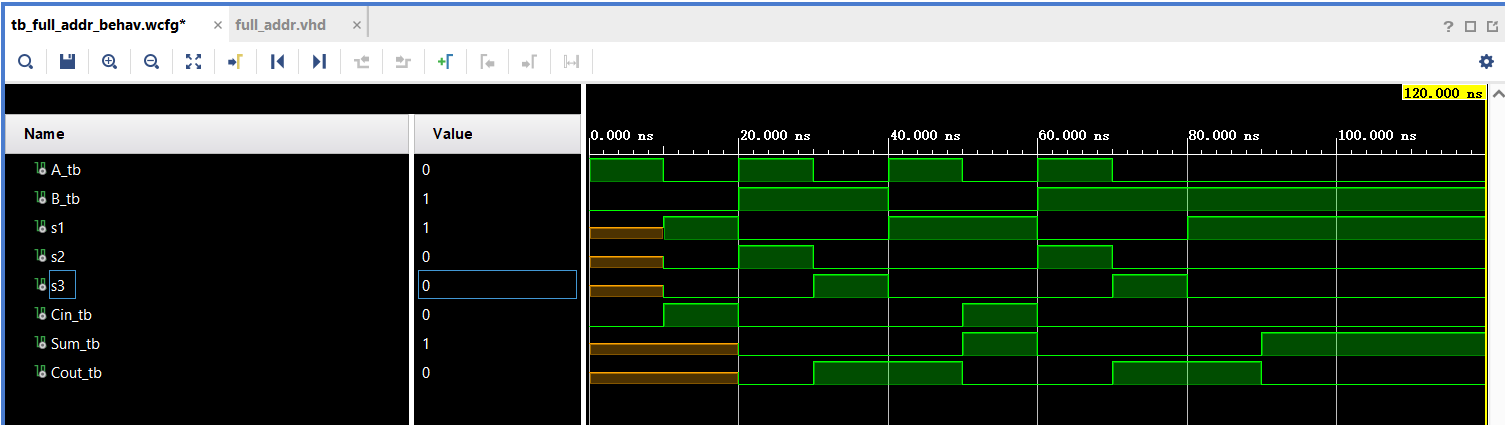
\includegraphics{D:/MyProjects/FPGA/Lab2/full_addr_report/assets/behav_sim.png}

The behavioral simulation result is the same as the previous manually
developed results (Figure TODO). If we look at the RTL schematic (Figure
TODO), we notice that the logic diagram is totally the same as Figure
TODO.

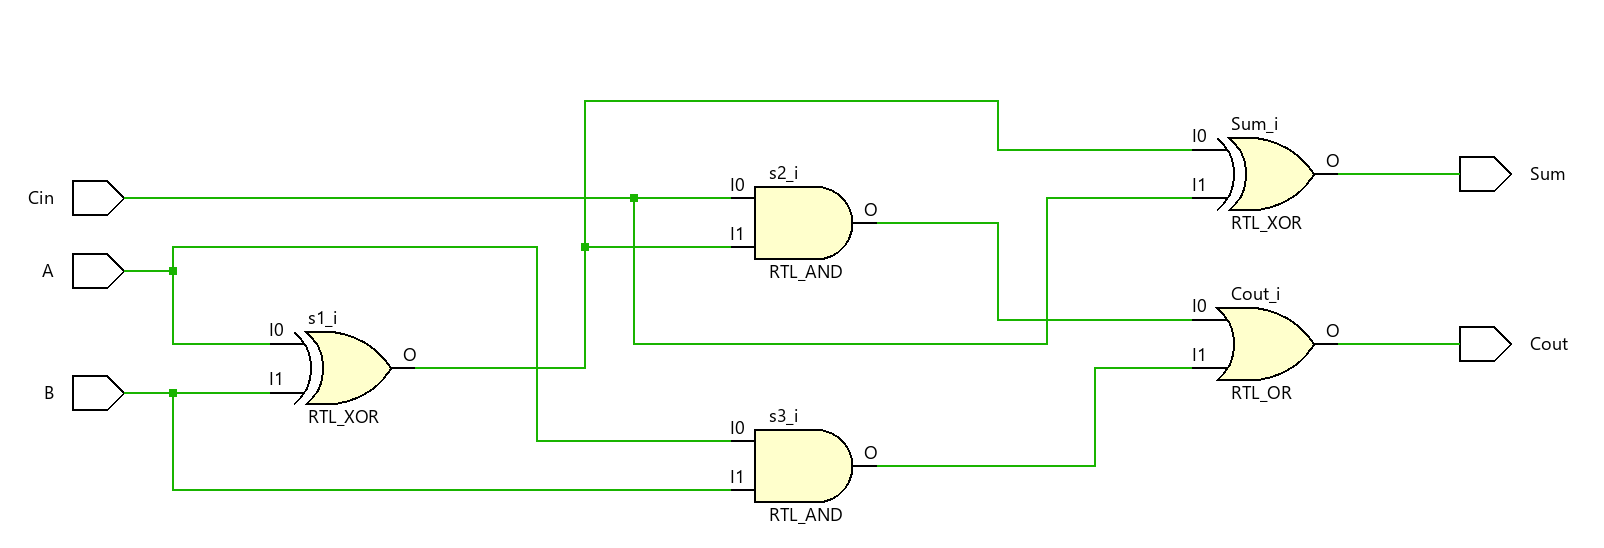
\includegraphics{D:/MyProjects/FPGA/Lab2/full_addr_report/assets/behav_schem.png}

However, due to the huge gate delay we set for the behavioral
simulation, the addition result is not consistent with our common sense,
since the input signals vary as quickly as the gate delay.

\textbf{To make it closer to our common sense}, we can simply modify the
gate delay to 0ns, and rerun the simulation. The result (Figure TODO) is
more like an intuitive full adder now.

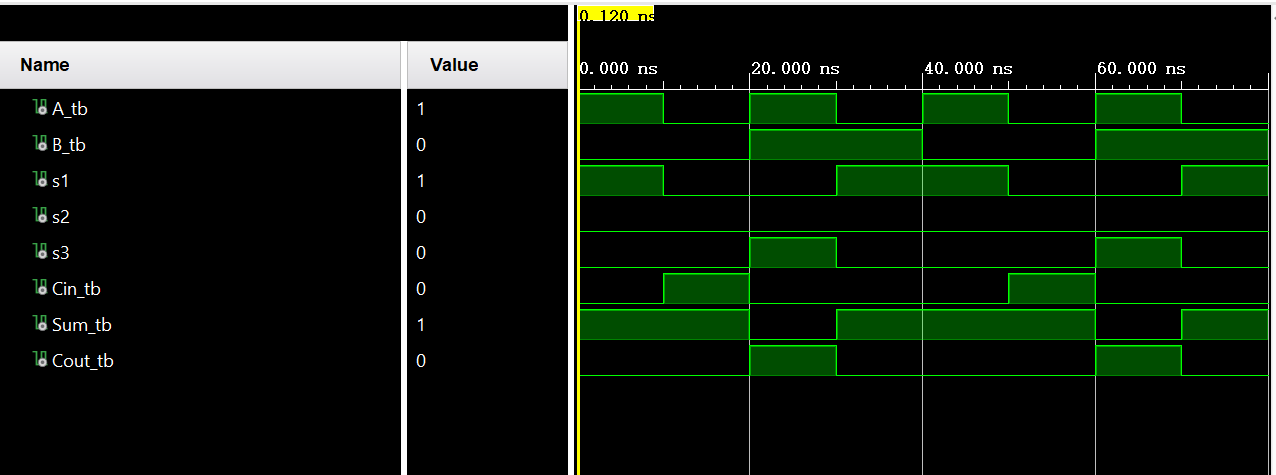
\includegraphics{D:/MyProjects/FPGA/Lab2/full_addr_report/assets/image-20240306203610995.png}

\hypertarget{post-synthesis-simulation}{%
\subsection{Post-Synthesis Simulation}\label{post-synthesis-simulation}}

The synthesis process transfers the design source to a physically
compatible design, regardless of the specific hardware board. Since
onboard devices mainly involve Look-up tables (LUTS) and use them to
fulfill combinational logic, it may have some performance differences
with that design directly using logic gates to accomplish. Moreover, the
synthesis process eliminates those unnecessary self-defined gate delays.
The schematic of the synthesis result (Figure TODO) doesn't resemble the
one in the previous RTL schematic (Figure TODO), showing the root cause
of the difference between the post-synthesis simulation and the
behavioral simulation.

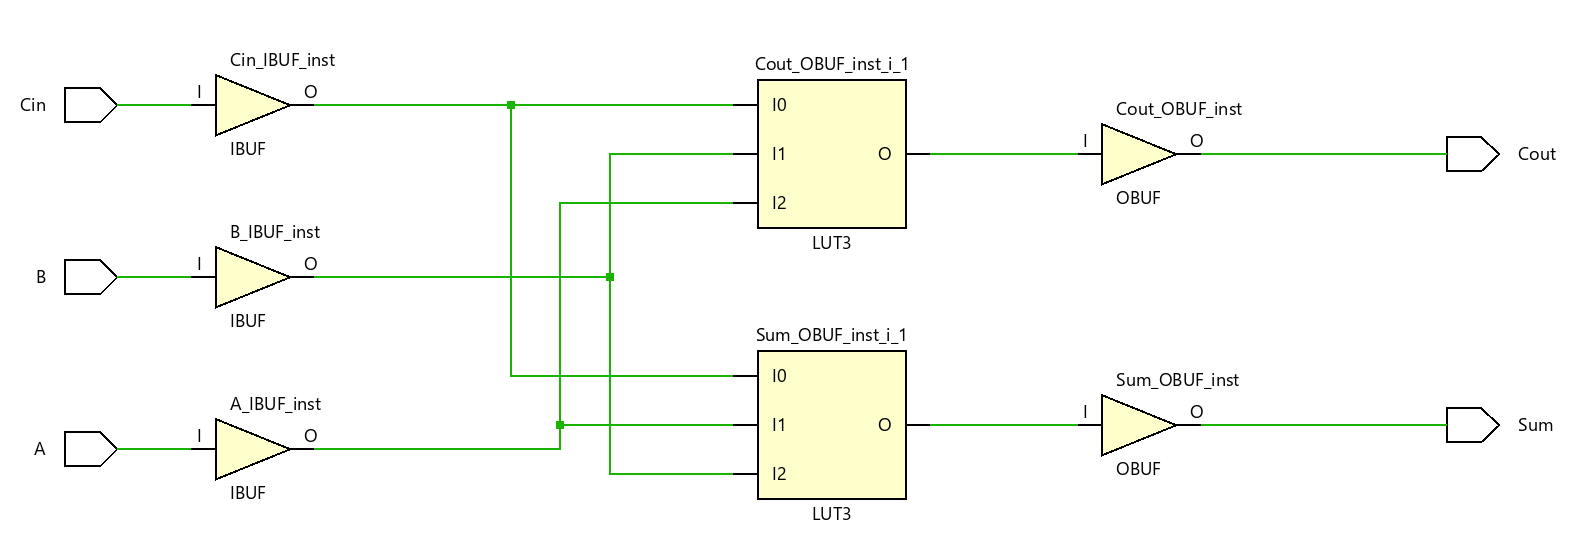
\includegraphics{D:/MyProjects/FPGA/Lab2/full_addr_report/assets/synth_schem.png}

\hypertarget{functional}{%
\subsubsection{Functional}\label{functional}}

Post-synthesis functional simulation eliminates all self-defined gate
delays as well as the actual gate delays. The result is as Figure TODO,
which is the same as the zero gate delay behavioral simulation, and it
is consistent with our common sense of a full adder.

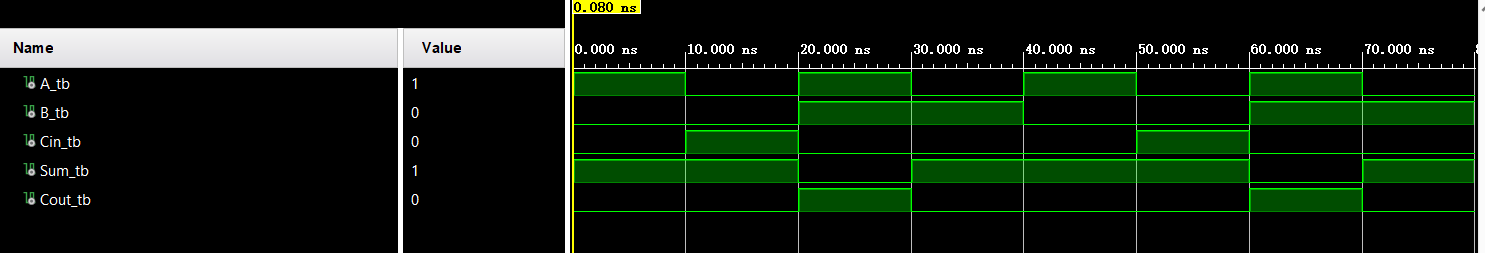
\includegraphics{D:/MyProjects/FPGA/Lab2/full_addr_report/assets/synth_func.png}

\textbf{Note:} Although the synthesis eliminates those self-defined gate
delays in the source design file (i.e. statement like
\texttt{after\ x\ ns}), the stimulus signals defined in the testbench
preserved the timing characteristic.

\hypertarget{timing}{%
\subsubsection{Timing}\label{timing}}

Post-synthesis timing simulation only differs from the functional
simulation in that it involves generally estimated gate delays (i.e.
gate delays in different devices are estimated the same). As shown in
Figure TODO, the output signals \texttt{Sum\_tb} and \texttt{Count\_tb}
are simply a constant time-delayed version of the functional simulation
as shown in Figure TODO.

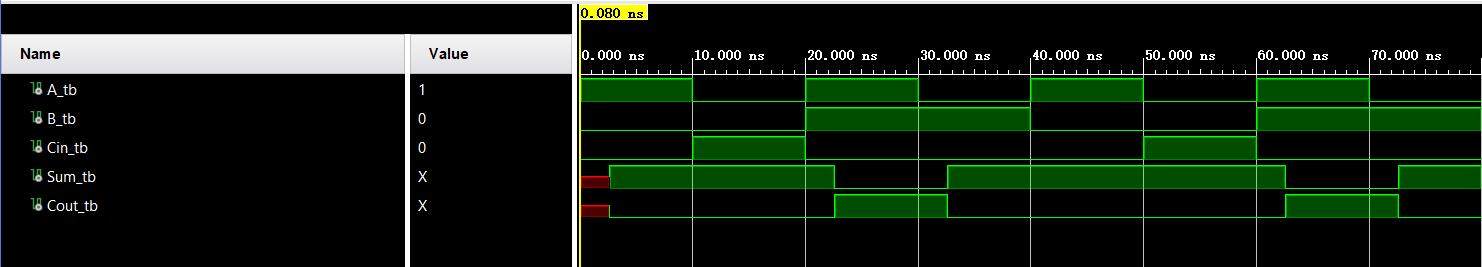
\includegraphics{D:/MyProjects/FPGA/Lab2/full_addr_report/assets/synth_tim.png}

\hypertarget{post-implementation-simulation}{%
\subsection{Post-Implementation
Simulation}\label{post-implementation-simulation}}

Post-implementation is also regarded as post-place-and-route simulation.
This type of simulation considered the actual hardware devices on board
as well as the wiring. However, in this lab, post-implementation
simulation is generally alike post-synthesis simulation. The schematic
of the implementation result (Figure TODO) is the same as the synthesis
result (Figure TODO).

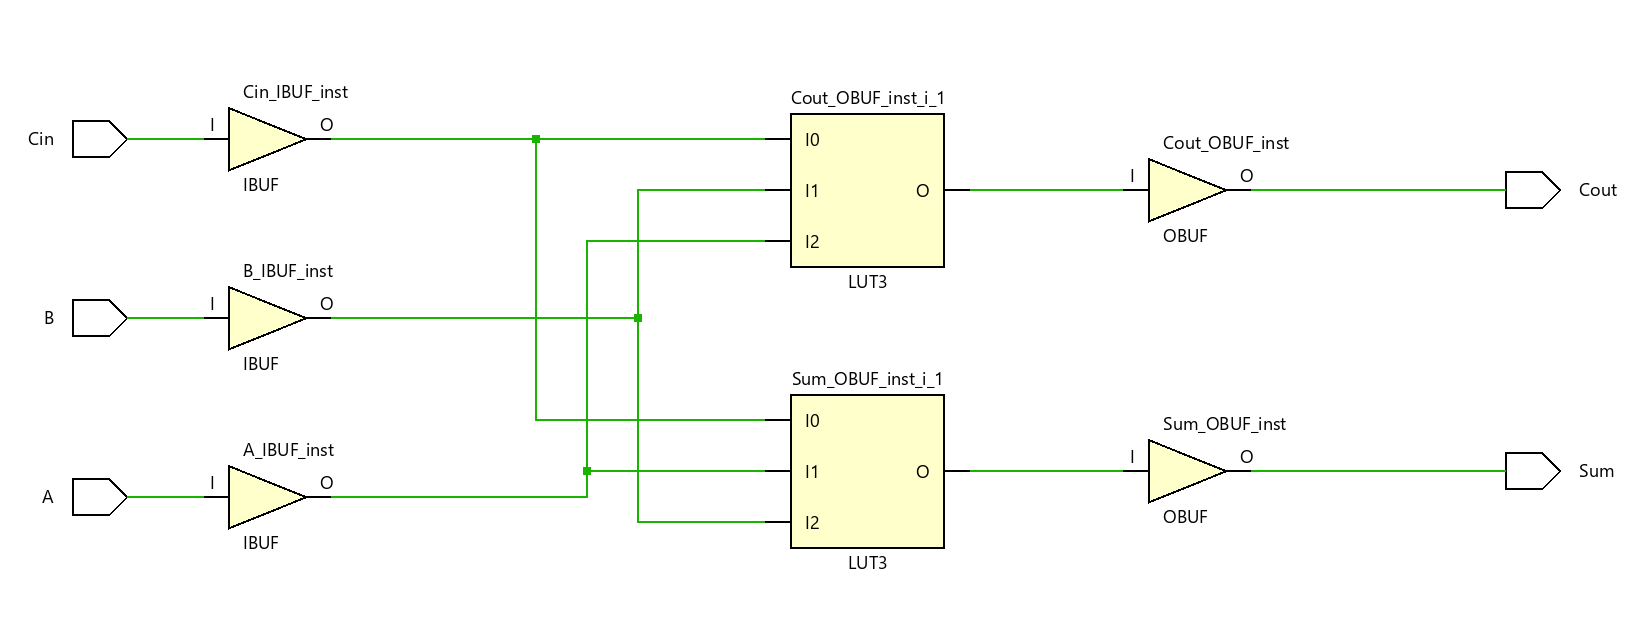
\includegraphics{D:/MyProjects/FPGA/Lab2/full_addr_report/assets/impl_schem.png}

\hypertarget{functional-2}{%
\subsubsection{Functional}\label{functional-2}}

The post-implementation functional simulation also ignores the
self-defined gate delays in the source design while preserving the
timing characteristic defined in the testbench. The simulation result
(Figure TODO) is consistent with our common sense as well as the
post-synthesis functional simulation.

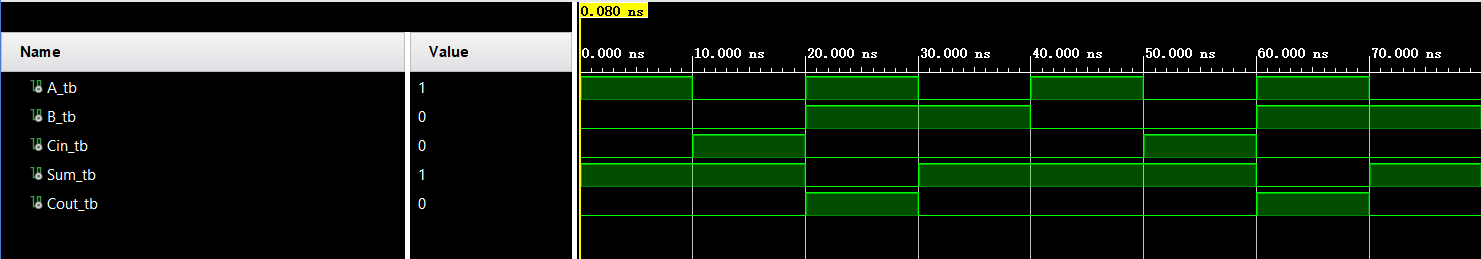
\includegraphics{D:/MyProjects/FPGA/Lab2/full_addr_report/assets/impl_func.png}

\hypertarget{timing-2}{%
\subsubsection{Timing}\label{timing-2}}

The most important part of the post-implementation timing simulation is
that it considers the actual gate delays of different devices and the
transport delay (i.e. delay due to the signal propagation in wires ), so
it can uncover some potential problems in our previous design. In this
lab, post-implementation timing simulation does do this job. As shown in
Figure TODO, there are a lot of spikes in the waveforms, which indicates
that the design exhibits \textbf{race hazard}. Race hazard is usually
due to the simultaneous variations of several input signals which can
result in opposite output.

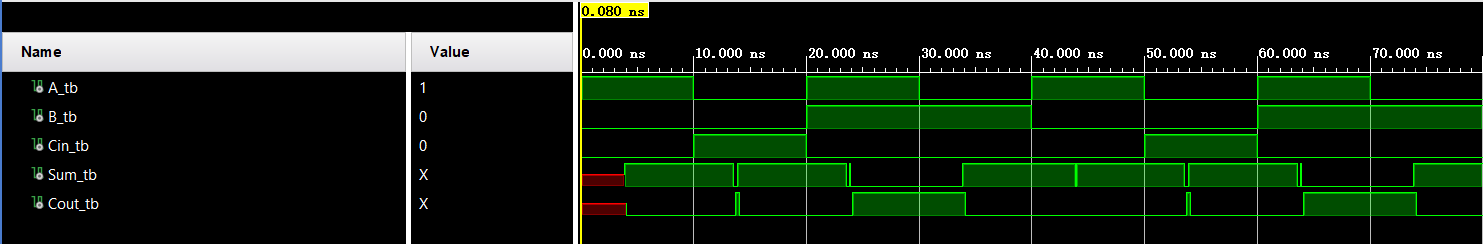
\includegraphics{D:/MyProjects/FPGA/Lab2/full_addr_report/assets/impl_tim.png}

\hypertarget{extension-eliminating-spikes-in-post-implementation-simulation}{%
\section{Extension: Eliminating Spikes In Post-Implementation
Simulation}\label{extension-eliminating-spikes-in-post-implementation-simulation}}

In the post-implementation timing simulation, we notice that there exist
spikes in the waveform. The implementation is done by placing devices
and routing wires on board, which can lead to different delays if the
signal takes on different paths. And this tiny delay difference can
result in spikes.

My core idea for eliminating the spikes is that we can add a clock
signal to drive the output, instead of making the full adder output
anytime. This can greatly reduce the potential of the full adder to
capture some transient states that exhibit singularity.

This idea needs the involvement of \textbf{D flip-flop}, which only
outputs the result when there is a rising edge of the clock signal.

In the design source, we need to add an input port of clock, and also
add a \texttt{when} statement at the output.

\begin{Shaded}
\begin{Highlighting}[]
\ControlFlowTok{entity} \DecValTok{full\_addr\_clk} \KeywordTok{is}
\ControlFlowTok{Port}\NormalTok{(}\OtherTok{...}
\NormalTok{	clk}\OtherTok{:} \KeywordTok{in} \DataTypeTok{STD\_LOGIC}\NormalTok{;}
	\OtherTok{...}\NormalTok{);}
\ControlFlowTok{end full\_addr\_clk;}
    
\ControlFlowTok{architecture} \DecValTok{dataflow} \KeywordTok{of} \FunctionTok{full\_addr\_clk} \KeywordTok{is}
    \OtherTok{...}
\KeywordTok{begin}
    \OtherTok{...}
\NormalTok{    L4}\OtherTok{:}\NormalTok{ sum }\OtherTok{\textless{}=}\NormalTok{ (s1 }\KeywordTok{xor}\NormalTok{ Cin) }\KeywordTok{after}\NormalTok{ gate\_delay }\KeywordTok{when} \KeywordTok{rising\_edge}\NormalTok{(clk);}
\NormalTok{    L5}\OtherTok{:}\NormalTok{ cout }\OtherTok{\textless{}=}\NormalTok{ (s2 }\KeywordTok{or}\NormalTok{ s3) }\KeywordTok{after}\NormalTok{ gate\_delay }\KeywordTok{when} \KeywordTok{rising\_edge}\NormalTok{(clk);}
    \OtherTok{...}
\ControlFlowTok{end architecture dataflow;}
\end{Highlighting}
\end{Shaded}

In the testbench, I added a clock source, which is a \texttt{process}:

\begin{Shaded}
\begin{Highlighting}[]
    \KeywordTok{process} \KeywordTok{is}
    \KeywordTok{begin}
        \KeywordTok{wait} \KeywordTok{for}\NormalTok{ 3ns;}
\NormalTok{        clk\_tb }\OtherTok{\textless{}=} \KeywordTok{not}\NormalTok{ clk\_tb;}
    \KeywordTok{end} \KeywordTok{process}\NormalTok{;}
\end{Highlighting}
\end{Shaded}

The period of 3ns is arbitrarily taken. However, if the period is set
too short, D flip-flops may not react correctly. And if the period is
set too long, the delay of the full adder then will be too large.

However, in my first experiment, I only found zero outputs of
\texttt{Sum\_tb} and \texttt{Count\_tb} in post-implement timing
simulation (Figure TODO), while all other functional simulations and
behavioral simulation accord with intuition.

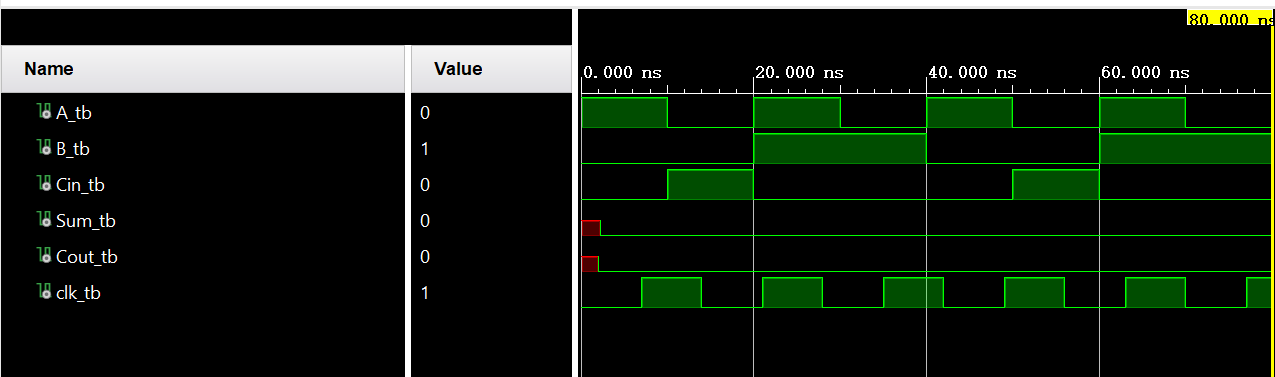
\includegraphics{D:/MyProjects/FPGA/Lab2/full_addr_report/assets/image-20240309215900176.png}

\textbf{So, I first establish my hypothesis that D flip-flops on this
board are not capable of handling this kind of rapid change of input
signal.} Thereafter, I extend all signals' duration tenfold in the
testbench and make the period of the clock to be 33ns.

Then I rerun the post-implementation simulation, and I found that while
the general shape of the waveform is satisfying (Figure TODO), the
\texttt{Sum\_tb} output is not consistent with the one in the previous
version (Figure TODO).

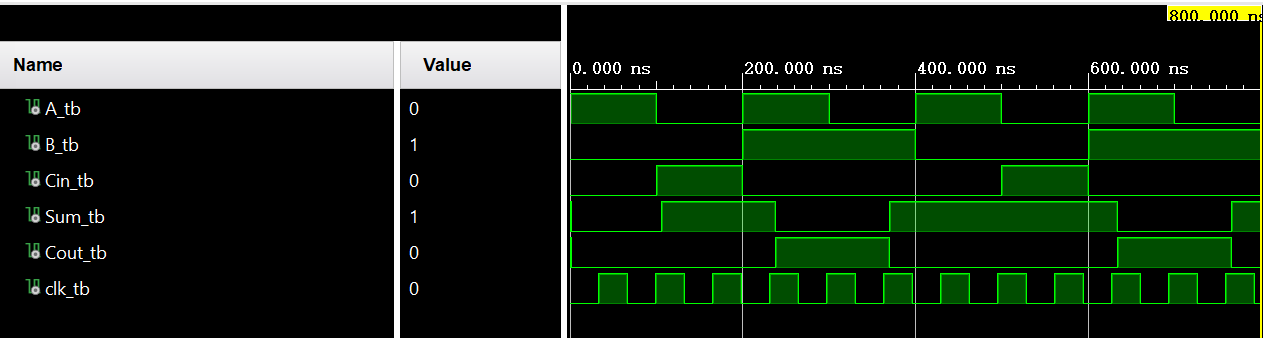
\includegraphics{D:/MyProjects/FPGA/Lab2/full_addr_report/assets/image-20240310155222394.png}

After tons of this kind of simulation with changing parameters, I found
a phenomenon in common, that is: the output signals don't vary at all
until around 100ns after the stimulus signals were fed into the system.

\textbf{Then I hypothesize that D flip-flops need more time to
initialize than LUTs, due to there may exist larger parasitic
capacitance in this kind of device, and the ``power-on initialization''
time is around 100ns.}

So then, I make the input signals (clock included) back to the original
state and repeat them twice. The post-implementation timing simulation
waveform is shown in Figure TODO.

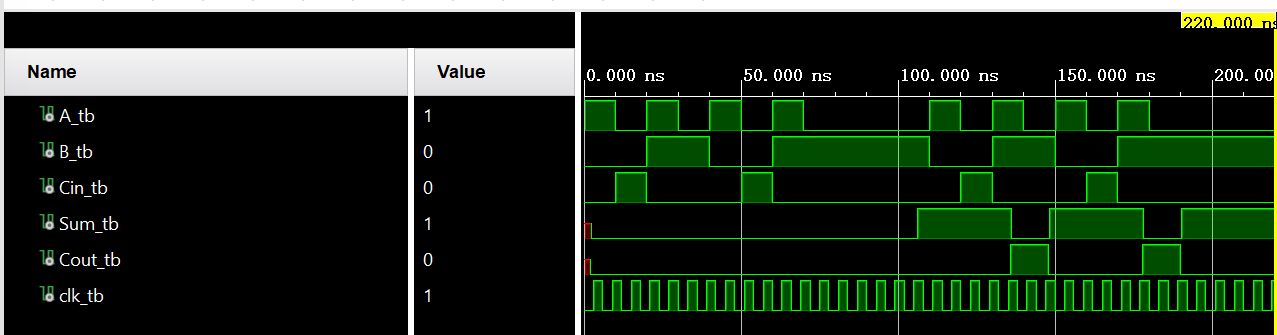
\includegraphics{D:/MyProjects/FPGA/Lab2/full_addr_report/assets/image-20240310161708176.png}

From Figure TODO, we can see that in the first cycle, the outputs are
all zeros. However, during the second cycle, all outputs are in accord
with our manual derivation with no spikes at all. And the period of the
clock can be as short as 3ns!

\hypertarget{conclusion}{%
\section{Conclusion}\label{conclusion}}

In this lab, we investigate the differences among the five types of
simulations. These simulations stand for each stage in which we carry
our design from a draft to a hardware-compatible one. As the simulation
proceeds, we can discover if our design can be carried out on physical
hardware. Post-synthesis simulation tells us how the logic gate will be
replaced by stuff like LUTs on hardware, and whether this design is
synthesizable. Then post-implementation simulation helps us uncover
potential problems that will happen on hardware. On top of that, we
delve deeper into the formation of spikes in post-implementation
simulation, and we develop a strategy of using clock-driven output to
eliminate unexpected spikes.

\hypertarget{appendix-full-code}{%
\section{Appendix: Full code}\label{appendix-full-code}}

\end{document}
